% Fig 1 — LoD verification planning pipeline (standalone TikZ)
\documentclass[tikz,border=3pt]{standalone}
\usepackage[T1]{fontenc}
\usepackage{helvet}
\renewcommand{\familydefault}{\sfdefault}
\usetikzlibrary{arrows.meta,positioning,fit,backgrounds,calc}

\definecolor{lodblue}{HTML}{1565C0}
\definecolor{lodorange}{HTML}{E65100}
\definecolor{lodpurple}{HTML}{6A1B9A}
\definecolor{lodgray}{HTML}{546E7A}
\definecolor{loddash}{HTML}{B0BEC5}

\tikzset{
  stage/.style={
    draw=#1, thick, rounded corners=2pt, fill=white,
    minimum height=7.5mm, minimum width=14mm, align=center,
    font=\footnotesize, inner sep=2pt
  },
  goal/.style={stage=#1, minimum width=17mm},
  arr/.style={-{Stealth[length=2mm]}, draw=lodgray, thick},
  arrD/.style={-{Stealth[length=2mm]}, draw=loddash, thick, dashed},
}

\begin{document}
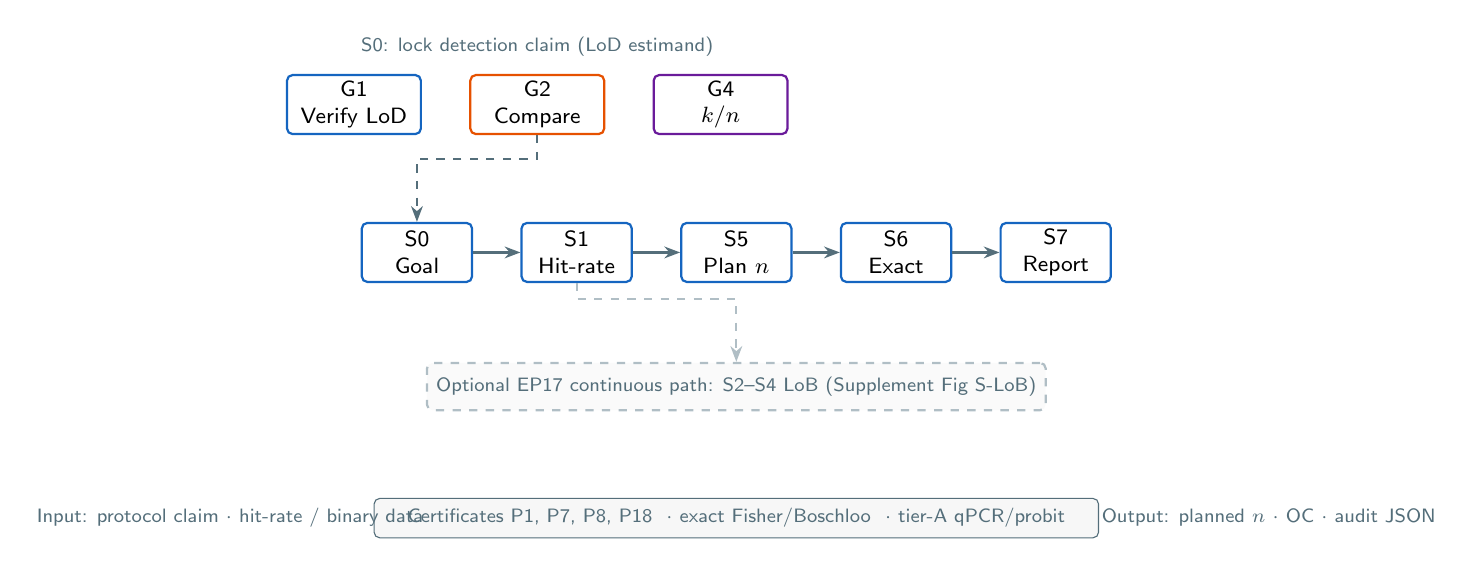
\begin{tikzpicture}[node distance=4mm and 6mm]

  % G1 / G2 / G4 (LoD scope)
  \node[goal=lodblue] (g1) {G1\\Verify LoD};
  \node[goal=lodorange, right=of g1] (g2) {G2\\Compare};
  \node[goal=lodpurple, right=of g2] (g4) {G4\\$k/n$};
  \node[above=1mm of g2, font=\scriptsize, text=lodgray] {S0: lock detection claim (LoD estimand)};

  % Main LoD pipeline
  \node[stage=lodblue, below=11mm of g1, xshift=8mm] (s0) {S0\\Goal};
  \node[stage=lodblue, right=of s0] (s1) {S1\\Hit-rate};
  \node[stage=lodblue, right=of s1] (s5) {S5\\Plan $n$};
  \node[stage=lodblue, right=of s5] (s6) {S6\\Exact};
  \node[stage=lodblue, right=of s6] (s7) {S7\\Report};
  \foreach \a/\b in {s0/s1,s1/s5,s5/s6,s6/s7}
    \draw[arr] (\a) -- (\b);

  \draw[arr, dashed] (g2.south) -- ++(0,-3mm) -| (s0.north);

  % Optional continuous / LoB branch (supplement)
  \node[draw=loddash, dashed, thick, rounded corners=2pt, fill=black!2,
        minimum width=42mm, minimum height=6mm, below=10mm of s5,
        font=\scriptsize, text=lodgray, align=center] (sup)
        {Optional EP17 continuous path: S2--S4 LoB (Supplement Fig S-LoB)};

  \draw[arrD] (s1.south) -- ++(0,-2mm) -| (sup.north);

  % Audit strip
  \node[draw=lodgray, fill=black!3, rounded corners=2pt,
        minimum width=92mm, minimum height=5mm,
        below=11mm of sup, font=\scriptsize, text=lodgray] (audit)
        {Certificates P1, P7, P8, P18 \ $\cdot$\ exact Fisher/Boschloo \ $\cdot$\ tier-A qPCR/probit};

  \node[font=\scriptsize, text=lodgray, anchor=west] at ([xshift=-44mm]audit.west)
        {Input: protocol claim $\cdot$ hit-rate / binary data};
  \node[font=\scriptsize, text=lodgray, anchor=east] at ([xshift=44mm]audit.east)
        {Output: planned $n$ $\cdot$ OC $\cdot$ audit JSON};

\end{tikzpicture}
\end{document}
